\documentclass[11pt]{article}
\usepackage[margin=1in]{geometry}
\usepackage[T1]{fontenc}
\usepackage[utf8]{inputenc}
\usepackage{lmodern}
\usepackage{setspace}
\usepackage{enumitem}
\usepackage{natbib}
\usepackage{tikz}
\usetikzlibrary{arrows.meta,positioning}

\title{Opposition--Load--Coupling (OLC): A Mechanistic Model of Internal Cognitive Agent Formation, Stabilization, and Dissolution}
\author{Anonymous Author}
\date{}

\begin{document}
\maketitle
\onehalfspacing

\begin{center}
\fbox{\parbox{0.95\linewidth}{
\textbf{Safety Note.} This paper analyzes a past cognitive event that occurred under unsafe conditions involving social isolation, emotional distress, and elevated cognitive load. It is a retrospective reconstruction, not a technique or method. The processes described here should not be intentionally replicated. Individuals experiencing similar symptoms should seek professional support.
}}
\end{center}

\begin{abstract}
This paper presents a retrospective single-subject case study of a self-constructed internal cognitive agent formed under prolonged social isolation and elevated cognitive stress. The Opposition--Load--Coupling (OLC) model formalizes a multi-stage mechanism: environmental preconditioning, construction via self-talk, opposition induction, cognitive load amplification, subconscious coupling, and emergent autonomy. A Shared Value Anchor is identified as a central stabilization mechanism that enables bounded cooperation between competing cognitive modules. The construct provided functional benefits in internal simulation and emotional regulation but introduced risks related to boundary degradation and cognitive interference. The agent was subsequently dismantled through deliberate disengagement, followed by a transition toward externally structured cognitive frameworks. This work proposes a descriptive mechanistic account of internal agent dynamics, defines stability conditions, and identifies risk amplification pathways in this case. The framework is exploratory, non-clinical, and not intended for replication.
\end{abstract}

\section{Introduction}
Internal dialogue enables humans to simulate alternative perspectives. Under constrained conditions---such as prolonged social isolation, reduced external feedback, and high internal cognitive demand---these simulations may differentiate into persistent agent-like structures. Internal dialogue and multi-voiced cognition have been studied in psychological theory \citep{hermans2001dialogical}, while dual-process cognition highlights interaction between controlled and automatic systems \citep{kahneman2011thinking}. Predictive-processing accounts further suggest that cognition operates through competing internal models \citep{friston2010free}.

This paper reconstructs a full lifecycle in one retrospective case: environmental preconditioning, construction, opposition, amplification, coupling, emergent autonomy, instability, dissolution, and post-agent transition. The objective is analytical rather than procedural: to understand boundary conditions, stabilization factors, and failure modes of internally constructed cognitive agents.

\textbf{Clinical boundary.} The OLC model does not diagnose, classify, or imply any psychiatric disorder. It is a cognitive-engineering reconstruction of internal dynamics within a unified cognitive system, and no clinical claims are made.

\section{Conceptual Framework}
\subsection{Internal Cognitive Agent}
An internal cognitive agent is defined here as a structured cognitive submodule capable of generating semi-independent responses and influencing internal reasoning while remaining embedded within a single cognitive system.

\subsection{Dynamic Boundary Condition}
The boundary between stable and destabilizing states is dynamic rather than fixed. Stability depends on three concurrent conditions: preserved meta-awareness of construct status, retained ability to regulate engagement, and demonstrated dissolvability. Instability emerges when these conditions degrade---for example, when module boundaries weaken, control becomes inconsistent, or construct influence intrudes into core decision processes.

\section{Methodology}
This study is a single-subject retrospective reconstruction based on long-horizon memory analysis and functional decomposition of cognitive processes. Events occurred several years before documentation, and no contemporaneous physiological or behavioral measurements were recorded.

Raw notes were post-hoc normalized into phase labels (Phase 0 to Phase V, then instability and dissolution stages) to reduce narrative drift and support transparent mapping from experience to model structure. This approach supports interpretability but does not provide causal proof.

The study is exploratory and non-generalizable. Claims are limited to descriptive dynamics observed in this case.

\section{The Opposition--Load--Coupling (OLC) Model}
\subsection{Phase 0: Environmental Preconditioning}
The process emerged under prolonged social isolation, low meaningful interpersonal interaction, and unmet demand for cognitive engagement. This configuration created sustained internal processing demand without adequate external regulation.

\subsection{Phase I: Construction via Self-Talk}
Repeated internal dialogue and deliberate reinforcement of an ``other perspective'' produced a proto-agent with increasing continuity across interactions.

\subsection{Phase II: Opposition Induction}
The proto-agent was intentionally positioned as an opposing module that generated disagreement, resistance, and counterarguments. This intervention reduced internal echo and created a stable dual-module tension.

\subsection{Phase III: Cognitive Load Amplification}
Elevated emotional intensity and sustained internal processing increased load. In this state, top-down control weakened relative to automatic associative activity, and response dynamics became less deliberately curated.

\subsection{Phase IV: Subconscious Coupling}
The core transition occurred when associative (subconscious) output streams were integrated into the opposition channel under reduced top-down filtering. A practical loop formed: primary module prompt $\rightarrow$ associative candidate generation $\rightarrow$ opposition-channel selection and expression. As coupling strengthened, responses appeared less directly authored and less predictable from conscious intention alone. This pattern is consistent with predictive-processing accounts in which reduced top-down precision weighting allows bottom-up associative signals to exert stronger influence \citep{friston2010free}.

\subsection{Phase V: Emergent Autonomy}
The system exhibited semi-independent response patterns, continuity across interactions, and reduced perceived direct control. In this model, autonomy is phenomenological (perceived autonomy), not ontological independence. The construct remained stimulus-responsive within internally generated prompts and did not show reliable independent initiation of interaction.

\begin{figure}[h]
\centering
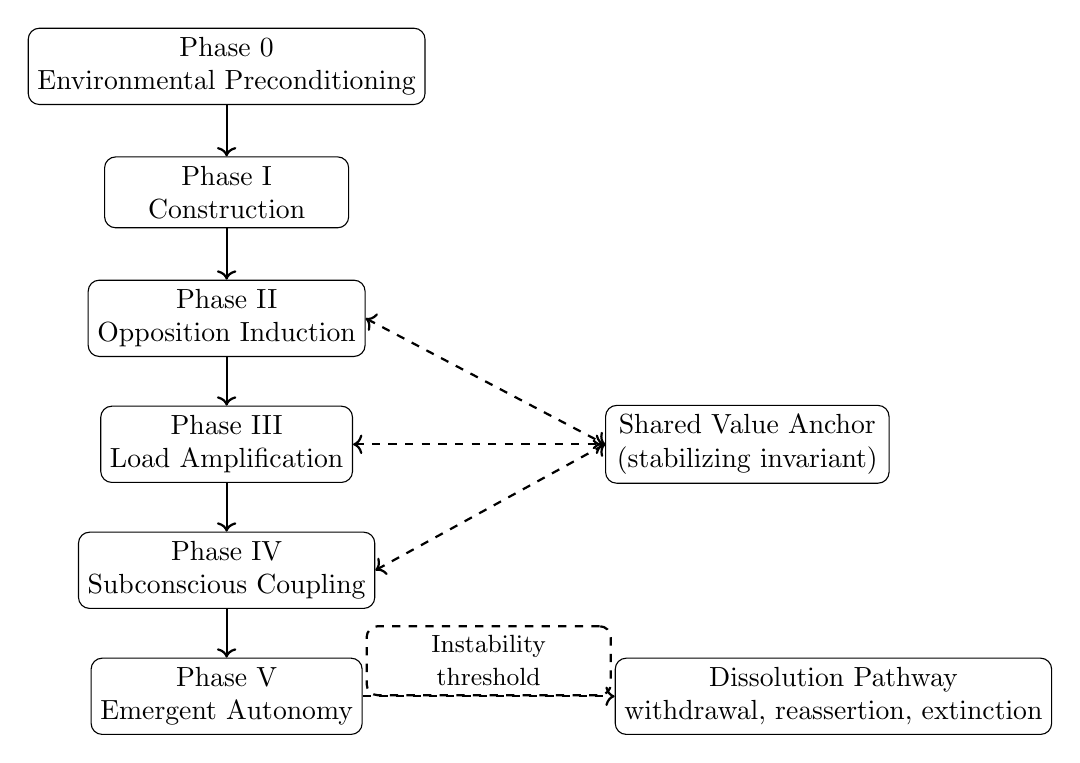
\begin{tikzpicture}[
    node distance=1.6cm,
    every node/.style={draw, rectangle, rounded corners, align=center, minimum width=3.1cm, minimum height=0.85cm},
    arrow/.style={->, thick}
]
\node (p0) {Phase 0\\Environmental Preconditioning};
\node (p1) [below of=p0] {Phase I\\Construction};
\node (p2) [below of=p1] {Phase II\\Opposition Induction};
\node (p3) [below of=p2] {Phase III\\Load Amplification};
\node (p4) [below of=p3] {Phase IV\\Subconscious Coupling};
\node (p5) [below of=p4] {Phase V\\Emergent Autonomy};
\node (anchor) [right=3.2cm of p3, minimum width=3.6cm] {Shared Value Anchor\\(stabilizing invariant)};
\node (diss) [right=3.2cm of p5, minimum width=3.6cm] {Dissolution Pathway\\withdrawal, reassertion, extinction};
\draw[arrow] (p0) -- (p1);
\draw[arrow] (p1) -- (p2);
\draw[arrow] (p2) -- (p3);
\draw[arrow] (p3) -- (p4);
\draw[arrow] (p4) -- (p5);
\draw[<->, thick, dashed] (p2.east) -- (anchor.west);
\draw[<->, thick, dashed] (p3.east) -- (anchor.west);
\draw[<->, thick, dashed] (p4.east) -- (anchor.west);
\draw[arrow, dashed] (p5.east) -- node[above, align=center] {\small Instability\\\small threshold} (diss.west);
\end{tikzpicture}
\caption{Opposition--Load--Coupling (OLC) stage model with anchor stabilization and dissolution branch}
\end{figure}

\section{Shared Value Anchor}
A shared value reference emerged between modules and acted as a stabilizing invariant. Mechanistically, this anchor constrained the objective space of both channels: disagreement could continue at the policy level, but not at the level of protected core value. As a result, conflict intensity remained bounded even when coupling was high.

This mechanism helps explain why opposition did not immediately collapse into full antagonism. The anchor preserved a minimum coordination channel, reduced full-system fragmentation, and supported recoverable interaction after spikes of internal conflict.

In systems terms, the anchor functioned similarly to a protected variable that competing processes preserve despite opposition. In dialogical-self terms, it can be interpreted as a shared organizing position that keeps internal voices in relation rather than in total dissociation \citep{hermans2001dialogical}.

\section{Functional Roles}
The key inversion is that functional benefits were valid only while boundary integrity remained stable. Within that window, the construct served as an internal simulation partner, an adversarial reasoning channel, and a temporary emotional-regulation support. It improved hypothesis stress-testing and perspective diversification.

Once boundaries degraded, the same mechanisms no longer produced net benefit. Opposition pressure began to spill into decision interference, and response variability shifted from useful exploration toward destabilizing noise.

\section{Instability and Risk}
Instability manifested through boundary degradation, intermittent control imbalance, and cognitive interference in decision flow. Risk was amplified by sustained high cognitive load and factors that increased perceptual or interpretive distortion.

In this case, late-stage instability included crisis-level deterioration and acute self-harm risk, indicating that failure modes were not merely conceptual but functionally severe. This inclusion is reported for model fidelity and safety framing, not for procedural detail. It further indicates that instability in this configuration can escalate beyond cognitive interference into dangerous functional states, reinforcing the necessity of boundary control and eventual dissolution.

To avoid diagnostic overreach, effects are described phenomenologically (for example, destabilized reality-monitoring and intrusive conflict carryover) rather than as clinical classification labels.

\section{Dissolution Process}
Dissolution required deliberate multi-step disengagement rather than spontaneous recovery. First, reinforcement was withdrawn by reducing or stopping participation in the opposition channel. Second, centralized control was reasserted by prioritizing unified decision processes. Third, opposition response continuity weakened and extinguished over time.

The aftereffect was mixed: long-term stability improved, while short-term loss of internal dialogue richness and a transient sense of cognitive emptiness were reported. Dissolution was therefore stabilizing but not affectively neutral.

\section{Post-Agent Transition}
After dissolution, cognition transitioned from internal agent-based processing toward externalized structured frameworks, including formal models and system-level abstraction. This shift reduced recurrence risk by moving high-load reasoning into auditable external artifacts.

\section{Implications}
The case contributes to cognitive engineering by showing how internal adversarial simulation can produce both analytical gains and stability hazards. It also offers a cross-domain analogy to multi-agent design: opposition can increase robustness, but only when bounded by invariant alignment constraints and reliable boundary controls.

\textbf{Broader significance.} Internal agent formation is relevant to multi-agent cognition, self-modeling, and boundary stability under load. These observations may inform future research in cognitive science, AI safety, and human--AI interaction, especially where competing internal objectives must remain coherent without losing operator control.

\section{Conclusion}
This retrospective case supports six descriptive conclusions: an internal agent-like structure was intentionally constructed in this case; OLC provides a coherent mechanism map for its lifecycle; Shared Value Anchor functioned as a stabilizer; instability followed boundary degradation; dissolution was achievable through systematic disengagement; and externalized frameworks offered more reliable long-term stability after transition.

These conclusions are case-bounded and non-generalizable. The contribution is a structured descriptive model and safety-oriented boundary account, not a clinical or procedural framework.
This analysis is descriptive only and should not be interpreted as a technique or intervention.

\section{Limitations}
The study is single-subject, retrospective, and memory-based, with no external instrumentation. Therefore, temporal precision is limited, latent confounders cannot be ruled out, and causal claims cannot be established. Observational claims in this paper concern the reconstructed sequence and phenomenology reported in this case. Hypothesis-level claims concern the proposed mechanism links between opposition, load, coupling, stabilization, and failure. What may generalize is a candidate structure of mechanisms and boundary conditions; what cannot be generalized from this record is prevalence, diagnostic mapping, or treatment implication.

\section{Future Work}
\begin{itemize}[leftmargin=*]
  \item Multi-subject validation under ethical oversight to test whether the phase sequence and boundary dynamics recur across cases with different backgrounds.
  \item Computational simulation of OLC transitions and boundary-failure thresholds to separate robust mechanisms from case-specific narrative factors.
  \item Formal integration with predictive-processing and dialogical-self research to improve theoretical interoperability and terminology precision.
  \item Development of non-replicative safety guidance focused on destabilization recognition and early disengagement decision criteria.
\end{itemize}

\bibliographystyle{plainnat}
\bibliography{references}

\end{document}
